
\documentclass[article]{IEEEtran}
\usepackage[a5paper, margin=10mm, onecolumn]{geometry}

\usepackage{tfrupee} 
\setlength{\headheight}{1cm} 
\setlength{\headsep}{0mm}       
\usepackage{multicol}
\usepackage{gvv-book}
\usepackage{gvv}
\usepackage{cite}
\usepackage{amsmath,amssymb,amsfonts,amsthm}
\usepackage{algorithmic}
\usepackage{graphicx}
\usepackage{textcomp}
\usepackage{xcolor}
\usepackage{txfonts}
\usepackage{listings}
\usepackage{enumitem}
\usepackage{mathtools}
\usepackage{gensymb}
\usepackage{comment}
\usepackage[breaklinks=true]{hyperref}
\usepackage{tkz-euclide} 
\usepackage{listings}

\def\inputGnumericTable{}                                 
\usepackage[latin1]{inputenc}                                
\usepackage{color}                                            
\usepackage{array}                                            
\usepackage{longtable}                                       
\usepackage{calc}                                             
\usepackage{multirow}                                         
\usepackage{hhline}                                           
\usepackage{ifthen}                                           
\usepackage{lscape}
\begin{document}
	\title{5.9.7}
	\author{EE25BTECH11052 - Shriyansh Kalpesh Chawda}
	\maketitle
\textbf{Question}\\
	A part of monthly hostel charges in a college hostel are fixed and the remaining depends on the number of days one has taken food in the mess. When a student A takes food for 25 days, he has to pay \rupee 4,500, whereas a student B who takes food for 30 days, has to pay \rupee 5,200. Find the fixed charges per month and the cost of
	food per day.\\

	\hfill{(10, 2019)}\\
	\textbf{Solution}\\
Let x be the fixed charge and y be the cost of food per day.\\
The system according to the information is
\begin{align}
	x + 25y &= 4500 \\
	x + 30y &= 5200
\end{align}
In matrix form:
\begin{align}
	\myvec{1 & 25 \\ 1 & 30} \myvec{x \\ y} = \myvec{4500 \\ 5200}.
\end{align}
Let
\begin{align}
	A = \myvec{1 & 25 \\ 1 & 30}, \quad \vec{b} = \myvec{4500 \\ 5200}.
\end{align}
Solving it using Gauss-Jordan elimination, we get
\begin{align}
	\left[\begin{array}{cc|c}
		1 & 25 & 4500 \\
		1 & 30 & 5200
	\end{array}\right]
	&\xrightarrow{R_2 \rightarrow R_2 - R_1}
	\left[\begin{array}{cc|c}
		1 & 25 & 4500 \\
		0 & 5 & 700
	\end{array}\right] \\
	&\xrightarrow{R_2 \rightarrow \tfrac{1}{5}R_2}
	\left[\begin{array}{cc|c}
		1 & 25 & 4500 \\
		0 & 1 & 140
	\end{array}\right] \\
	&\xrightarrow{R_1 \rightarrow R_1 - 25R_2}
	\left[\begin{array}{cc|c}
		1 & 0 & 1000 \\
		0 & 1 & 140
	\end{array}\right]
\end{align}
From the reduced row echelon form, we have the solution:
\begin{align}
	\myvec{x \\ y} = \myvec{1000 \\ 140}
\end{align}

Therefore,
\begin{align}
	x = 1000 \quad \text{(fixed charge)}, \qquad y = 140 \quad \text{(cost per day)}.
\end{align}

\begin{figure}[H]
	\centering
	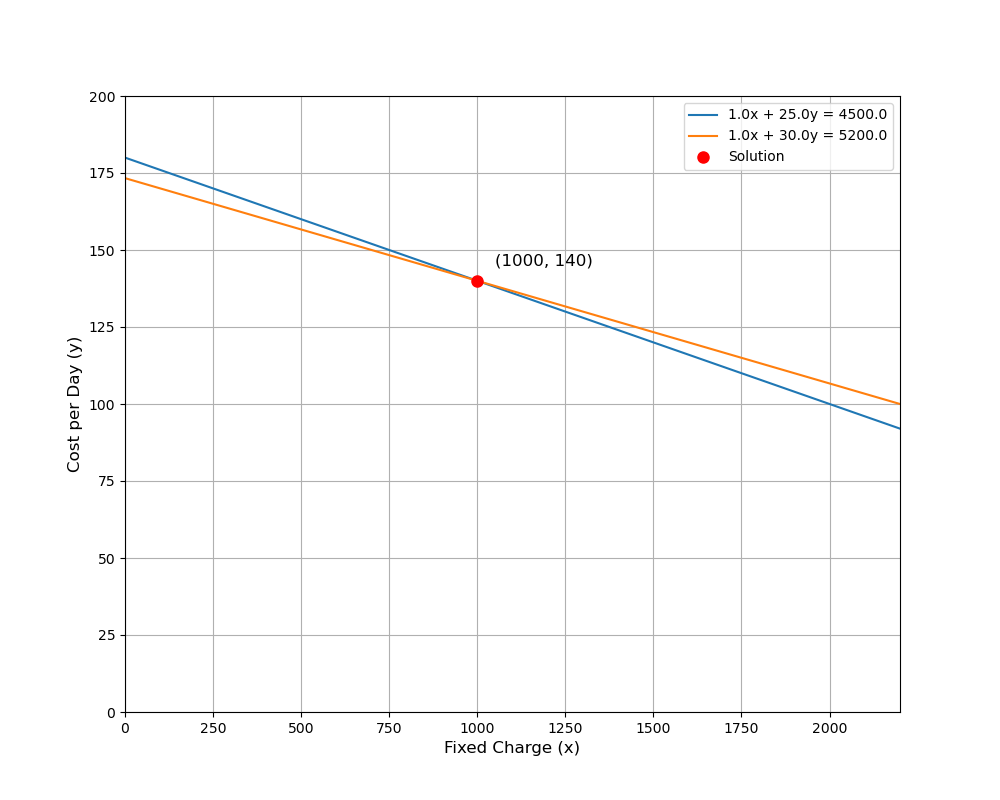
\includegraphics[width=1.1\linewidth]{figs/hostel_charges_plot}
\end{figure}

	
\end{document}